%This is a LaTeX template for homework assignments
\documentclass{article}
\usepackage[utf8]{inputenc}
\usepackage{amsmath}
\usepackage{float}
\usepackage{graphicx}
\usepackage{multicol}
\usepackage[spanish,es-nodecimaldot]{babel}
\usepackage{parskip}
\usepackage{algorithm}
\usepackage{url}
\usepackage{listings}
\usepackage{algpseudocode}
\usepackage{geometry}
\usepackage{amssymb}
\usepackage{dsfont}
\geometry{ top=17mm, bottom=16mm, left=15mm, right=15mm }
\begin{document}
\title{\vspace{-1cm}Deep Learning}
\author{Miguel Vilchis}
\date{}
\maketitle
\section{Definiciones generales}
  \begin{itemize}
    \item Recordar que el objetivo que tiene deep learning es encontrar 
    la función que logra clasificar correctamente cada entrada.
    \item Funciones de activación: Se usan funciones no lineales para
    poder aprender funciones no lineales.
    \item Parametrización: Proceso de definir que parametros son
    necesarios para un modelo dado.
    \item Función de perdida: Cuantifica que tan bien la clase de
    salida se apega a la verdadera clase. (Buscamos minimizar dicha
    función)
    \item Función de Scoring: Esta función acepta los datos como
    entrada y los mapea a una etiqueta de clase. Ejemplo: 
    \[ f(x_i, W, b) = Wx_i+b
    \] 
    Donde: 
    \begin{lstlisting}
    W = [K x D], x_i = [D x 1] y b = [K x 1]
    \end{lstlisting}
    Siendo K el número de clases para clasificar.
    \item Bias: Permite recorrer o transladar nuestra función de
    scoring en una u otra dirección sin modificar la matriz de pesos.
    \item Epoca: Cada vez que una red neuronal ha visto el conjunto completo 
    de entrenamiento se dice que una época ha pasado. 
  \end{itemize}
\section{Función de perdida}
  Es común usar funciones \textit{hinge} pero se usa mas 
  \textit{cross-entropy loss} y \textit{softmax} en el contexto de
  deep learning y redes convolucionales.
  \begin{itemize}
      \item Multi-class svm loss \\
       Se puede agregar la columna de Bias a la matriz de peso, con este truco, podemos
       dejar de preocuparnos por actualizar el bias, para solo parametrizar la matriz
       de pesos, haciendo esto nuestra función queda expresada como:
       \[
       s = f(x_i, W) = Wx_i
       \]
       Dado el punto \textit{i-esimo}, el score predicho de la clase \textit{jth} queda definido como:
       \[
       s_j = f(x_i, W)_j
       \]
       De aquí obtenemos la función \textit{hinge loss function}
       (sumando las clasificaciones incorrectas de cada clase y
       comparandola con la salida de la función score):
       \[
         L_i = \sum_{j \neq y_i} max(0, s_j - s_{y_i}+1)
       \]
       Mientras que la función \textit{squared hinge loss} penaliza
       mas la perdida y se define como:
       \[
         L_i = \sum_{j \neq y_i} max(0, s_j - s_{y_i}+1)^2
        \]
    \item Cross-entropy loss: Mientras la funcón softmax  regresa probabilidades 
    para cada clase. La función  \textit{hinge} nos da el margen. El
    clasificador softmax es la generalización de la forma binaria de la regresión
    logística. $f(x)_i = e^{s_{x_i}}/\sum_{j}e^{x_j}$ y la función de perdida \textit{cross-entropy}
    \[
    L_i = -ln(e^{s_{y_i}}/\sum_{j}e^{y_j})
    \]
    Entonces, la función de perdida debe minimizar el logaritmo negativo de la
    probabilidad de la clase correcta: 
    \[
    L_i = -lnP(Y=y_i|X=x_i) 
    \]
    Donde 
    \[
    P(Y=y_i|X=x_i) = e^{s_{y_i}}/\sum_j e^{s_j}
    \]
    Por lo que la función de perdida \textit{cross-entropy}
    \[
    L = \frac{1}{N} \sum_{i=1}^N L_i
    \]
\end{itemize}
\section{Descenso de gradiente}
Nosotros tratamos las superficies de perdida como convexas incluso si no lo son, ya que el hacerlo así 
da buenos resultados. El algoritmo de descenso de gradiente tiene dos veritentes:
\begin{enumerate}
    \item La implementación estandart \textit{vanilla}
    \item La versión optimizada \textit{estocástica}
\end{enumerate}
El pseudocodigo del descenso de gradiente es:
 \begin{lstlisting}
  while True:
   Wgradient = evaluate_gradient(loss, data, W)
   W += -alpha *Wgradient
 \end{lstlisting}
Para el gradiente estocástico, en lugar de calcular el gradiente para todo el conjunto de datos, se hace sobre un sampleo de estos. 
 \begin{lstlisting}
  while True:
   batch = next_training_batch(data, 256)
   Wgradient = evaluate_gradient(loss, data, W)
   W += -alpha *Wgradient
 \end{lstlisting}
\section{Momentum}
La idea es que, cuando estas descendiendo, este descenso te otorgué impulso para llegar más rápido (en menos épocas) 
a tener menor pérdida y mejor precisión. Sea $W = W - \alpha \bigtriangledown_{W} f(W)$ el termino V momentum, 
ponderado por $\gamma$: 
\[
  V = \gamma V_{t-1} + \alpha \bigtriangledown_{W} f(W)  \longrightarrow W = W - V_t
\]
Comunmente se usa $\gamma = 0.9$
\section{Regularización}
Es la técnica que asegura que nuestro modelo generalice bien, 
ayudandonos a controlar la capacidad de nuestro modelo. Lo cual logramos al penalizar altos valores de peso
,ya que, estos influyen más en la predicción de salida. Sea la función de perdida \textit{cross-entropy} $L$
\[
L_i = -log(e^{s_{y_i}}/ \sum_je^{s_j}) \longrightarrow L = \frac{1}{N}\sum{i=1}^N L_i
\]
La función de regularización o decaemiento del peso se define como: 
\[
R(W) = \sum_i \sum_j W_{i,j}^2
\]
Actualizando la función de perdida: 
\[
L = \frac{1}{N}\sum{i=1}^N L_i + \lambda R(W)
\]
Entonces: 
\[
W = W - \alpha \bigtriangledown_W f(W) -\lambda R(W)
\]
Tipos de regularización:
\begin{enumerate}
    \item L2 o decaemiento de peso: $R(W)= \sum_i \sum_j W_{i,j}^2$
    \item L1: $R(W)= \sum_i \sum_j |W_{i,j}|$
\end{enumerate}
\section{Función de activación}
Una vez que aplicamos la función de scoring, para determinar si la neurona se enciende o no utilizamos una función de
activación.
\begin{itemize}
 \item Función \textit{sigmoid}: Esta función es una buena opción ya que es continua y diferenciable donde sea, es simetrica
 en en eje y tiene una aproximación asintótica a los valores de saturación (0,1).\\
 Los grandes problemas de la función son: La salida no está centrada en 0 y las neuronas saturadas matan el gradiente 
 ya que los delta son extremadamente pequeños.
 \begin{figure}[H]
  \centering
  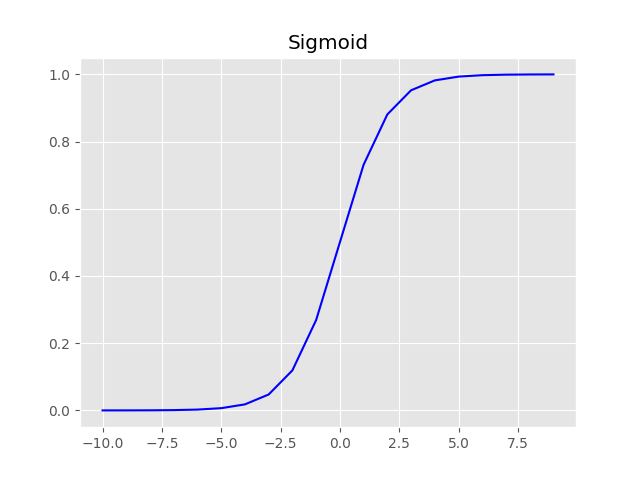
\includegraphics[width=0.3\textwidth]{images/Sigmoid.png}
  \caption{Función: $s(t) = \frac{1}{1+e^{-t}}$}
  \end{figure}
 \item Función \textit{tanh}: Es una función centrada en 0, pero el gradiente sigue siendo eliminado con neuronas 
  saturadas: 
 \begin{figure}[H]
  \centering
  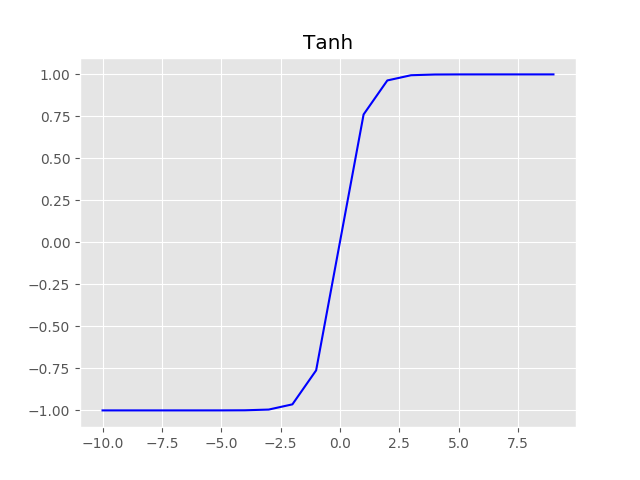
\includegraphics[width=0.3\textwidth]{images/Tanh.png}
  \caption{Función: $s(t) = \frac{e^t -e^{-t} }{e^{t}+e^{-t}}$}
 \end{figure}
 \item Función \textit{ReLU}: Es la función de activación más popular en deeplearning, el problema que tiene 
 es que con valores cercanos a 0, el gradiente no puede ser tomado. 
 \begin{figure}[H]
  \centering
  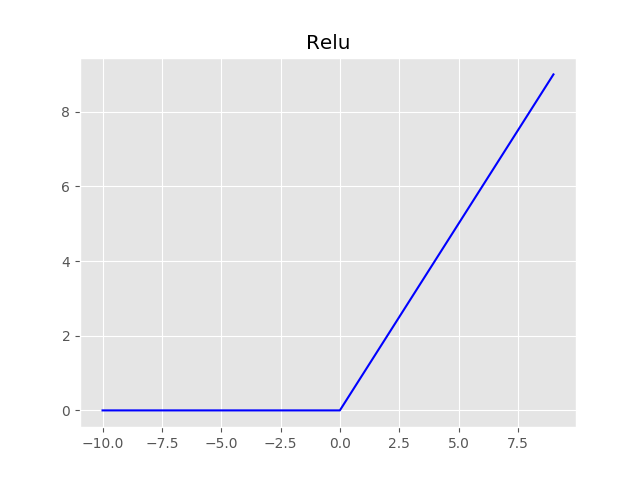
\includegraphics[width=0.3\textwidth]{images/Relu.png}
  \caption{Función: $s(t) = max(0,t)$}
 \end{figure}
 \item Función \textit{Leaky ReLU}: Es una variante de \textit{ReLU} que permite tomar gradientes cercanos a 0, diferentes 
 de cero. 
 \[ s(t) = \left \{ 
               \begin{array}{cc}
                t &  Si\ t \geq 0 \\
                \alpha \ \text{x}\  t &  En \ otro \ caso
               \end{array}
           \right .
  \]   
 \begin{figure}[H]
  \centering
  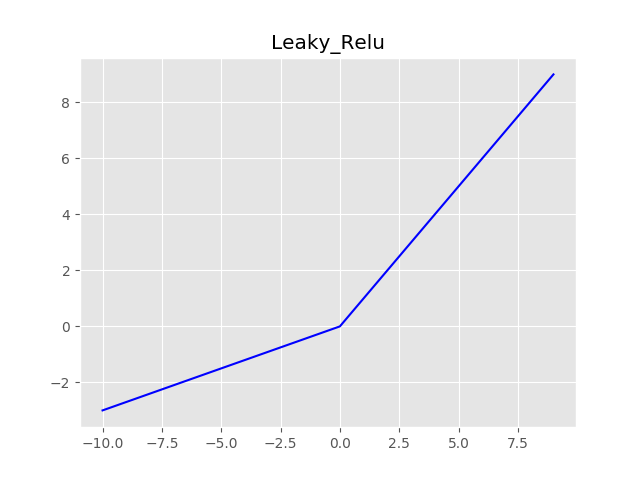
\includegraphics[width=0.3\textwidth]{images/Leaky_Relu.png}
  \caption{Grafica con $\alpha = 0.3$}
 \end{figure}

\item Functión \textit{Exponential Linear Units (ELU)}: Función que surge de un articulo del 2015
(\textit{Fast and Accurate Deep Learning by Exponential Linear Units}), en donde 
se obtienen mejor presición que con la función  $ReLU$, $ELU$ rara vez tiene peor desempeño que $ReLU$ (Usualmente se 
usa un valor de $\alpha$ cercano a 1.0)
 \[ s(t) = \left \{ 
               \begin{array}{cc}
                t &  Si\ t \geq 0 \\
                \alpha \ \text{x}\ (e^{t}-1) &  En \ otro \ caso
               \end{array}
           \right .
  \]   
 \begin{figure}[H]
  \centering
  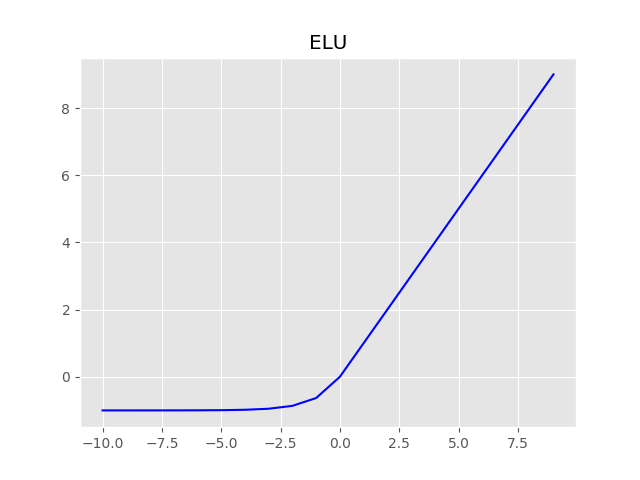
\includegraphics[width=0.3\textwidth]{images/ELU.png}
  \caption{Grafica con $\alpha = 1.0$}
 \end{figure}
\end{itemize}


\end{document}

